\documentclass[a4paper,12pt]{article}

\usepackage[utf8]{inputenc}
\usepackage[spanish]{babel}
\usepackage{amsmath, amssymb}
\usepackage{graphicx}
\usepackage{float}
\usepackage{booktabs}
\usepackage{xcolor}
\usepackage{listings}
\usepackage{caption}
\usepackage{fancyhdr}
\usepackage{hyperref}
\usepackage{tikz}

\hypersetup{
    colorlinks=true,
    linkcolor=blue,
    urlcolor=blue,
    pdftitle={Práctica 1 - OLED PWM},
}

% === Definición de colores similares a Vivado ===
\definecolor{vivadoKeyword}{rgb}{0.6,0.0,0.6}
\definecolor{vivadoComment}{rgb}{0.0,0.5,0.0}
\definecolor{vivadoString}{rgb}{0.5,0.2,0.0}
\definecolor{vivadoBackground}{rgb}{0.97,0.97,0.97}

\lstdefinelanguage{VHDL}{
    morekeywords={library, use, entity, is, port, in, out, end, architecture, of, begin, signal, if, then, else, when, others, xor, and, or, not},
    sensitive=true,
    morecomment=[l]--,
    morestring=[b]",
}

\lstset{
    language=VHDL,
    backgroundcolor=\color{vivadoBackground},
    keywordstyle=\color{vivadoKeyword}\bfseries,
    commentstyle=\color{vivadoComment}\itshape,
    stringstyle=\color{vivadoString},
    basicstyle=\ttfamily\small,
    numbers=left,
    numberstyle=\tiny,
    numbersep=5pt,
    frame=single,
    breaklines=true,
    tabsize=2,
    captionpos=b
}

\title{Práctica N°1: Medicion de Corriente con ajuste de PWM visualizado en OLED}
\date{}

\begin{document}
\maketitle
\tableofcontents
\newpage


\section{Objetivos}

\subsection*{Objetivo General}
Implementar un sistema embebido en la tarjeta \textbf{STM32F407G-DISC1} con la \textbf{Discovery Shield}, que permita la medición de corriente mediante un sensor de pasillo o Hall, el control de una señal PWM para la regulación de un motor mediante pulsantes y la visualización de datos en una pantalla OLED.

\subsection*{Objetivos Específicos}
\begin{itemize}
    \item Configurar el entorno de desarrollo \textbf{STM32CubeIDE} y realizar la correcta inicialización de los periféricos necesarios (SPI, TIM, GPIO y UART).
    \item Adquirir y procesar la señal de un \textbf{sensor de corriente digital} a través de la interfaz SPI.
    \item Generar y controlar una señal \textbf{PWM} mediante los temporizadores del microcontrolador para regular la velocidad de un motor de corriente continua.
    \item Implementar la comunicación y control gráfico de una \textbf{pantalla OLED SSD1351} para mostrar la corriente medida y el estado del PWM.
    \item Integrar todos los módulos desarrollados en un único proyecto funcional sobre la placa STM32F407G-DISC1.
    \item Validar experimentalmente el correcto funcionamiento del sistema, verificando la relación entre la corriente medida, el control PWM y la visualización en la pantalla.
\end{itemize}


\section{Desarrollo}


\subsection{Asignación de Pines en el STM32CubeMX}

Una parte fundamental en la configuración de un proyecto en STM32CubeIDE es la asignación de pines dentro del archivo \texttt{.ioc}. Cada periférico del microcontrolador debe conectarse correctamente a los pines físicos de la tarjeta de desarrollo.  

En esta práctica se requiere configurar los periféricos de la \textbf{pantalla OLED}, el \textbf{sensor de corriente Hall}, el \textbf{PWM para el control de motor}, el \textbf{driver de potencia} y los \textbf{pulsadores de control}.  

\subsubsection{Pines para la Pantalla OLED (SPI1)}

La pantalla OLED \textbf{SSD1351} se conecta al microcontrolador mediante la interfaz \textbf{SPI1} y pines adicionales de control:  

\begin{itemize}
    \item \textbf{PB5}: SPI1\_MOSI
    \item \textbf{PB4}: SPI1\_MISO
    \item \textbf{PB3}: SPI1\_SCK
    \item \textbf{PE5}: GPIO Output (Chip Select de la OLED)
    \item \textbf{PE4}: GPIO Output (RST de la OLED)
    \item \textbf{PB1}: GPIO Output (D/C de la OLED)
    \item \textbf{PD2}: GPIO Output (EN de la OLED)
\end{itemize}

Pines reseteados en esta etapa para evitar conflictos: \textbf{PE1, PB9, PB6, PB3, PD4, PC12, PC10}.  

\begin{center}
    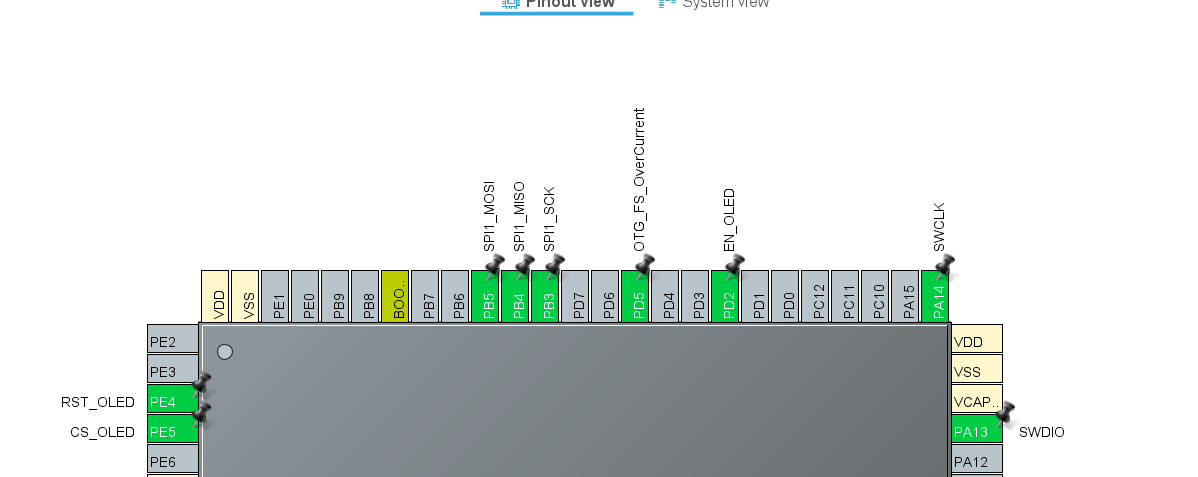
\includegraphics[width=0.8\textwidth]{Pines/OLED.png}
    \captionof{figure}{Configuración de pines para la pantalla OLED en el archivo \texttt{.ioc}.}
\end{center}

\subsubsection{Pines para el Sensor de Corriente Hall (SPI2)}

El sensor de corriente digital (\textbf{TLI4970}) se comunica mediante la interfaz \textbf{SPI2}:  

\begin{itemize}
    \item \textbf{PB15}: SPI2\_MOSI
    \item \textbf{PB14}: SPI2\_MISO
    \item \textbf{PB13}: SPI2\_SCK
    \item \textbf{PB12}: GPIO Output (Chip Select del sensor Hall)
\end{itemize}

Pines reseteados en esta etapa: \textbf{PA12, PA11, PA10, PA9, PC7}.  

\begin{center}
    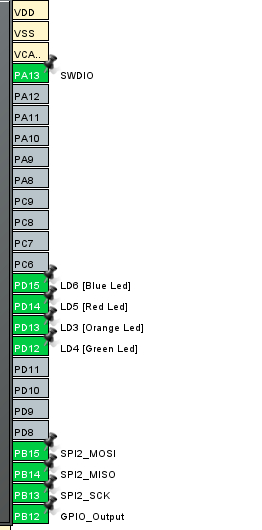
\includegraphics[width=0.4\textwidth]{Pines/Hall.png}
    \captionof{figure}{Configuración de pines para el sensor Hall en el archivo \texttt{.ioc}.}
\end{center}

\subsubsection{Pines para el PWM (TIM1)}

El control PWM se genera con el temporizador \textbf{TIM1}, cuya salida principal se conecta en:  

\begin{itemize}
    \item \textbf{PE13}: TIM1\_CH3 (PWM para el control del motor)
\end{itemize}

\begin{center}
    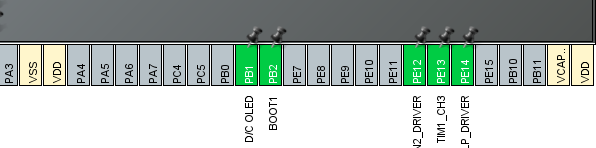
\includegraphics[width=0.8\textwidth]{Pines/driver.png}
    \captionof{figure}{Configuración del pin de salida PWM en el archivo \texttt{.ioc}.}
\end{center}

\subsubsection{Pines para el Driver de Motor}

El driver \textbf{TB6549FG} requiere tres señales de control adicionales:  

\begin{itemize}
    \item \textbf{PE14}: GPIO Output (SLP, habilitación del driver)
    \item \textbf{PE12}: GPIO Output (IN2)
    \item \textbf{PC2}: GPIO Output (IN1)
\end{itemize}



\subsubsection{Pines para los Pulsadores de Control}

Se emplean dos pulsadores conectados a entradas GPIO\_EXIT configuradas como interrupciones externas:  

\begin{itemize}
    \item \textbf{PA1}: GPIO External Interrupt (disminuye el valor del PWM)
    \item \textbf{PA2}: GPIO External Interrupt (aumenta el valor del PWM)
\end{itemize}

\begin{center}
    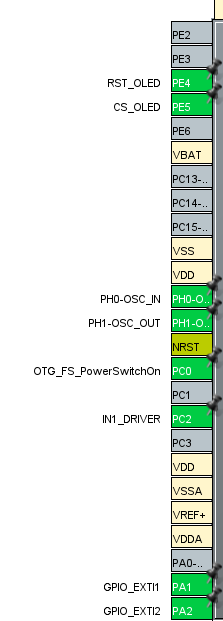
\includegraphics[width=0.4\textwidth]{Pines/pulsantes.png}
    \captionof{figure}{Configuración de pines para los pulsadores de control del PWM.}
\end{center}

\subsubsection{Modo de Reseteo de Pines}

En CubeMX, cada pin del microcontrolador puede asignarse a una función periférica, a un GPIO o quedar en estado de \textbf{Reset State}.  
El \textbf{modo Reset} significa que el pin permanece en su estado por defecto (alta impedancia o sin función asignada), evitando interferencias con otros periféricos.  

Para resetear un pin en CubeMX:
\begin{enumerate}
    \item Seleccionar el pin correspondiente en el diagrama del microcontrolador.
    \item En el menú emergente, escoger la opción \textbf{Reset State}.
    \item Verificar en la lista de pines (Pinout \& Configuration) que el pin ya no está asignado a ninguna función activa.
\end{enumerate}

\begin{center}
    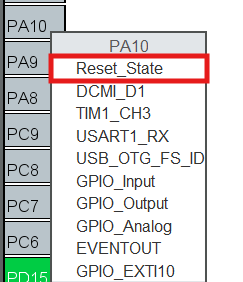
\includegraphics[width=0.7\textwidth]{Pines/reset.png}
    \captionof{figure}{Proceso de reseteo de pines en CubeMX.}
\end{center}

\subsection{Configuración de Periféricos en CubeMX}

Una vez asignados los pines, el siguiente paso consiste en configurar los periféricos en la pestaña \textbf{Configuration} del archivo \texttt{.ioc}. Esta etapa permite definir parámetros esenciales como la velocidad de comunicación, los modos de operación y la inicialización de cada módulo.

\subsubsection{Configuración de SPI1 (Pantalla OLED)}

La pantalla OLED basada en el controlador SSD1351 se comunica a través de la interfaz \textbf{SPI1}.  

Los parámetros recomendados son:
\begin{itemize}
    \item \textbf{Mode}: Full-Duplex Master.
    \item \textbf{Prescaler}: 8 (para obtener una frecuencia de reloj adecuada a la OLED).
    \item \textbf{Data Size}: 8 Bits.
    \item \textbf{Clock Polarity (CPOL)}: Low.
    \item \textbf{Clock Phase (CPHA)}: 1 Edge.
    \item \textbf{First Bit}: MSB First.
\end{itemize}

\begin{center}
    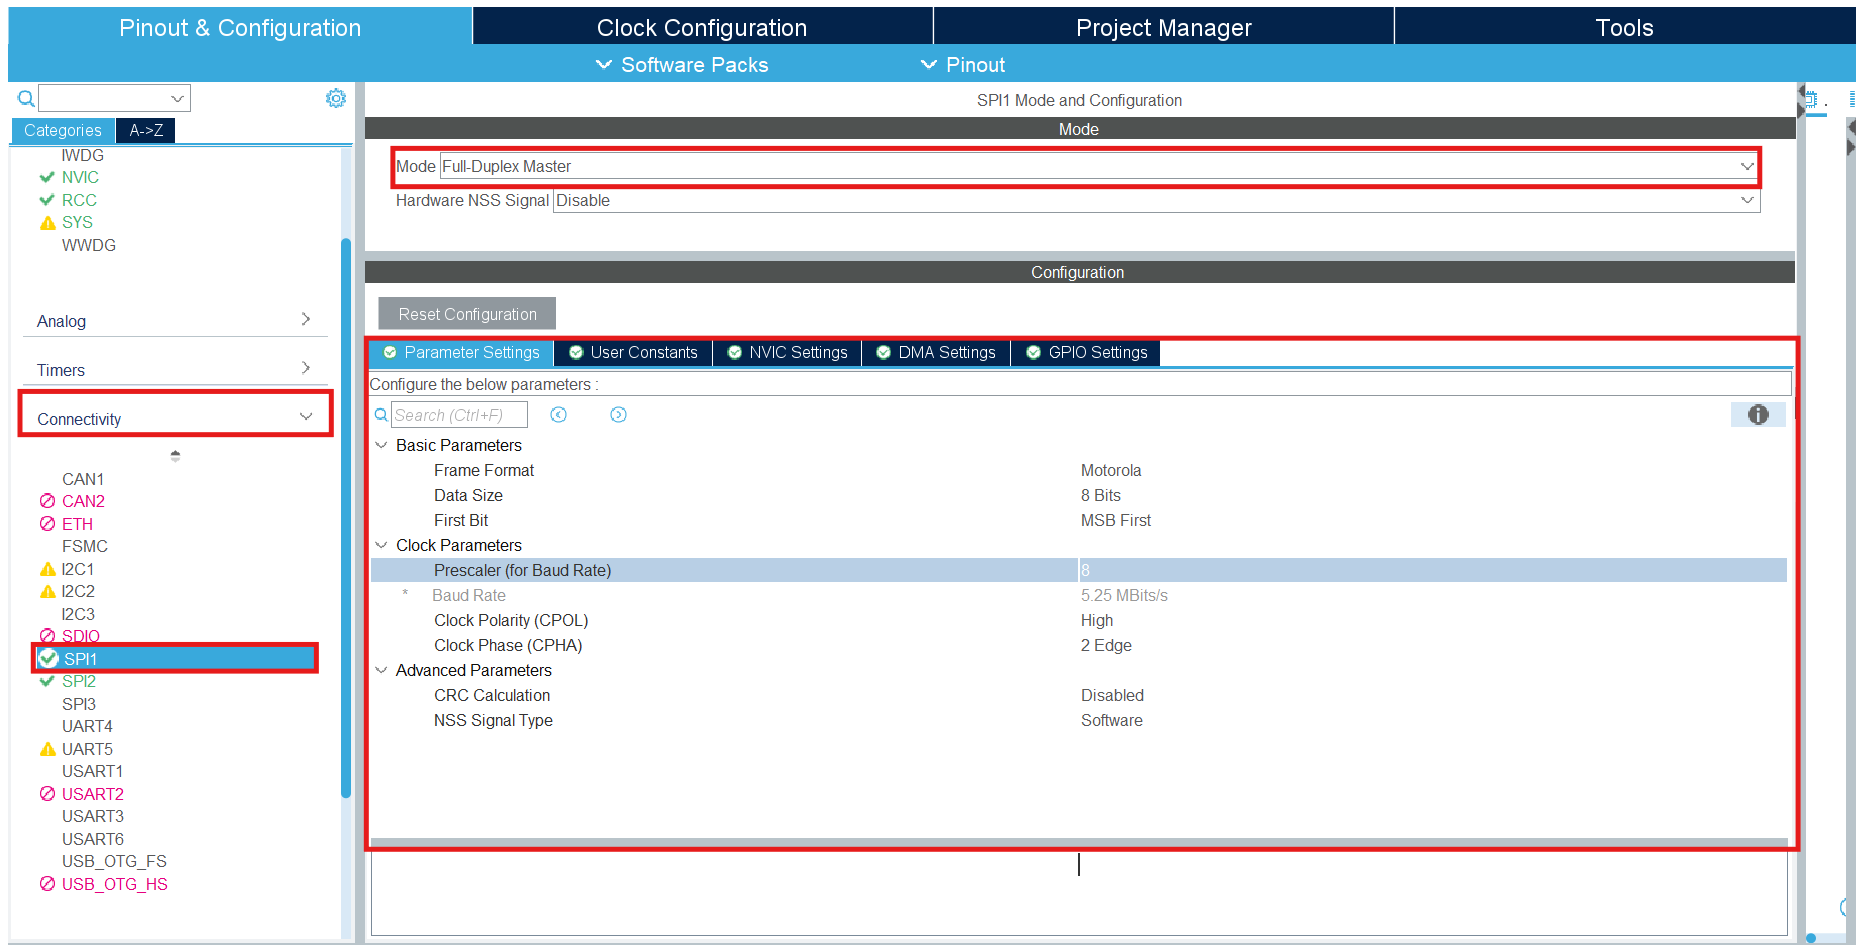
\includegraphics[width=0.75\textwidth]{Perifericos/oled.png}
    \captionof{figure}{Configuración de SPI1 para la comunicación con la pantalla OLED.}
\end{center}

\subsubsection{Configuración de SPI2 (Sensor Hall)}

El sensor de corriente TLI4970 emplea la interfaz \textbf{SPI2}. Su configuración es similar a SPI1, pero puede requerir un prescaler más bajo dependiendo de la velocidad de lectura deseada.

\begin{itemize}
    \item \textbf{Mode}: Full-Duplex Master.
    \item \textbf{Prescaler}: 16.
    \item \textbf{Data Size}: 8 Bits.
    \item \textbf{CPOL}: High.
    \item \textbf{CPHA}: 2 Edge.
    \item \textbf{First Bit}: MSB First.
\end{itemize}

\begin{center}
    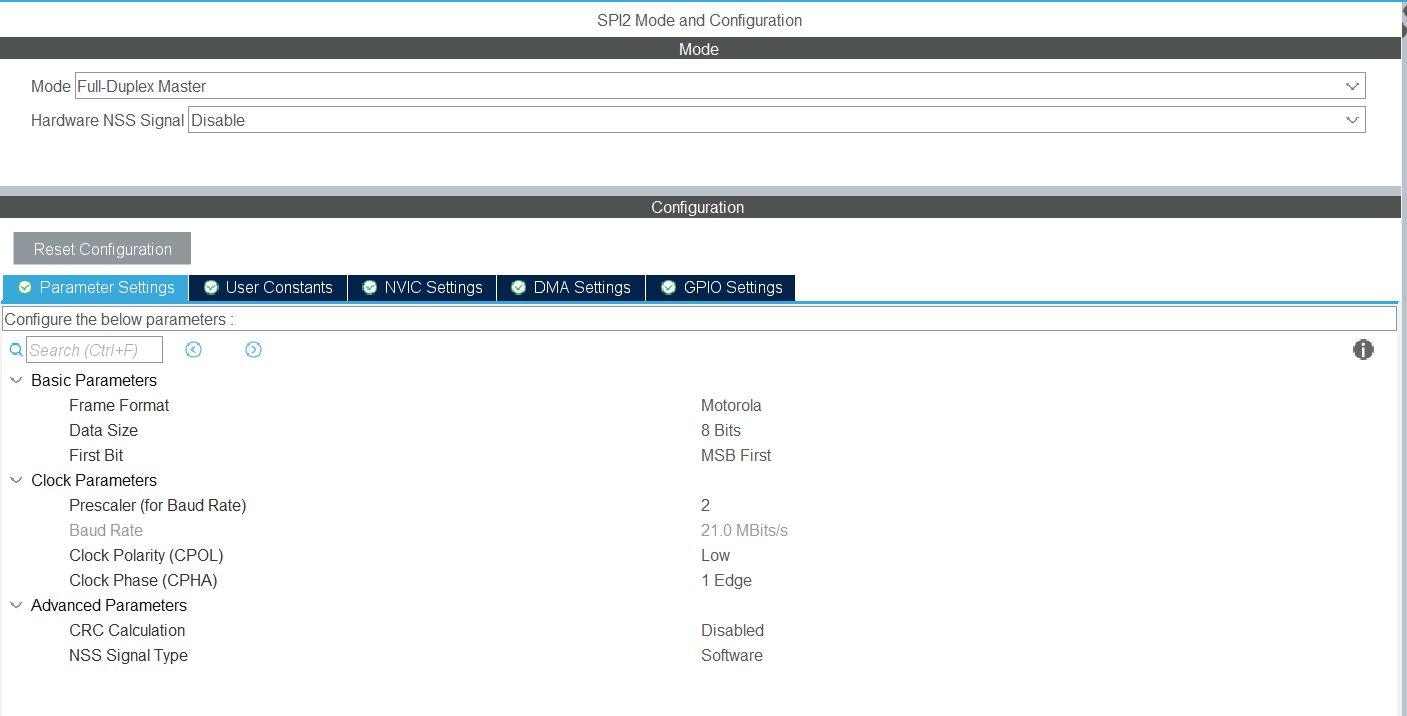
\includegraphics[width=0.75\textwidth]{Perifericos/hall.png}
    \captionof{figure}{Configuración de SPI2 para el sensor de corriente Hall.}
\end{center}

\subsubsection{Configuración de TIM1 (PWM)}

El \textbf{TIM1} se utiliza para generar la señal PWM que controla la velocidad del motor.  

Parámetros a configurar:
\begin{itemize}
    \item \textbf{Channel 3}: PWM Generation CH3 (activo en PE13).
    \item \textbf{Prescaler}: 83 (para dividir la frecuencia de reloj de 84 MHz).
    \item \textbf{Counter Period}: 999 (resolución de 1000 pasos, corresponde a 1 kHz de frecuencia de PWM).
    \item \textbf{PWM Mode}: PWM Mode 1.
    \item \textbf{Pulse}: valor inicial de duty cycle (ej. 100).
\end{itemize}

\begin{center}
    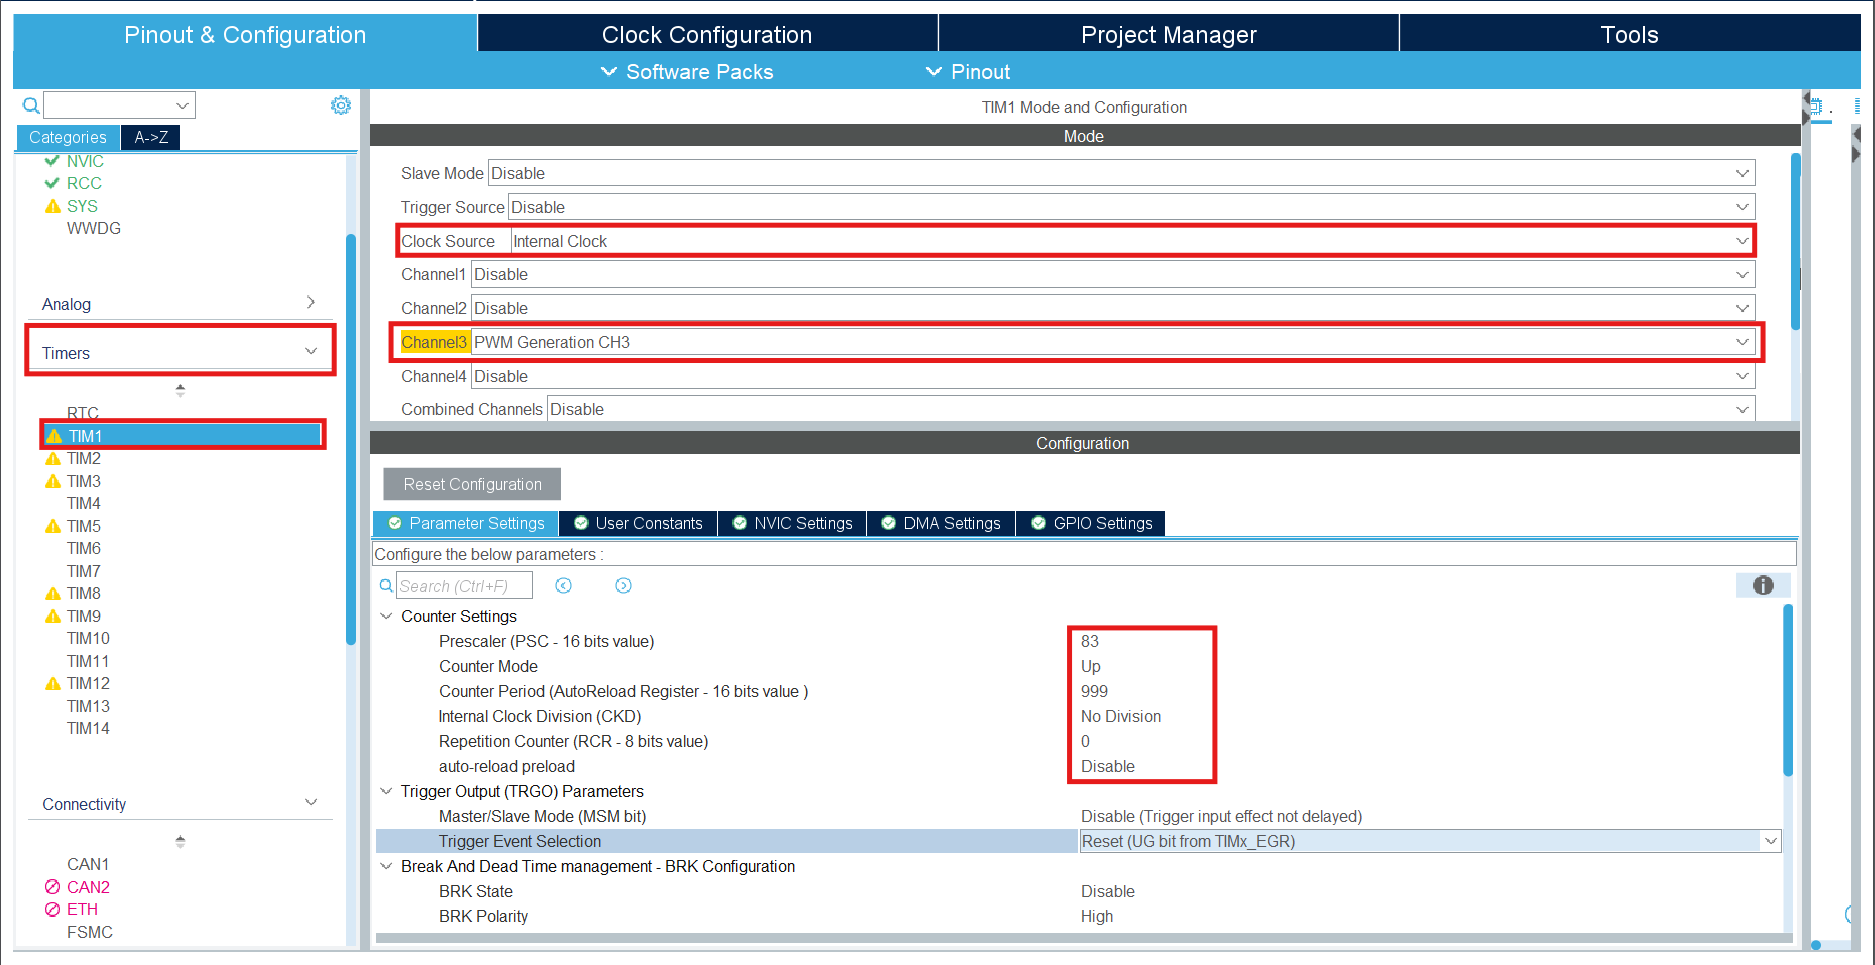
\includegraphics[width=0.75\textwidth]{Perifericos/timer.png}
    \captionof{figure}{Configuración de TIM1 para la generación de la señal PWM.}
\end{center}

\subsubsection{Configuración de GPIOs}

Los pines de control de la OLED y del driver de motor deben configurarse como \textbf{GPIO Output}:

\begin{itemize}
    \item \textbf{OLED}: PE5 (CS), PE4 (RST), PB1 (D/C), PD2 (EN).
    \item \textbf{Driver de Motor}: PE14 (SLP), PE12 (IN2), PC2 (IN1).
\end{itemize}

Modo de configuración:
\begin{itemize}
    \item Mode: Output Push-Pull.
    \item Pull-up/Pull-down: No pull.
    \item Maximum Output Speed: High.
\end{itemize}

\begin{center}
    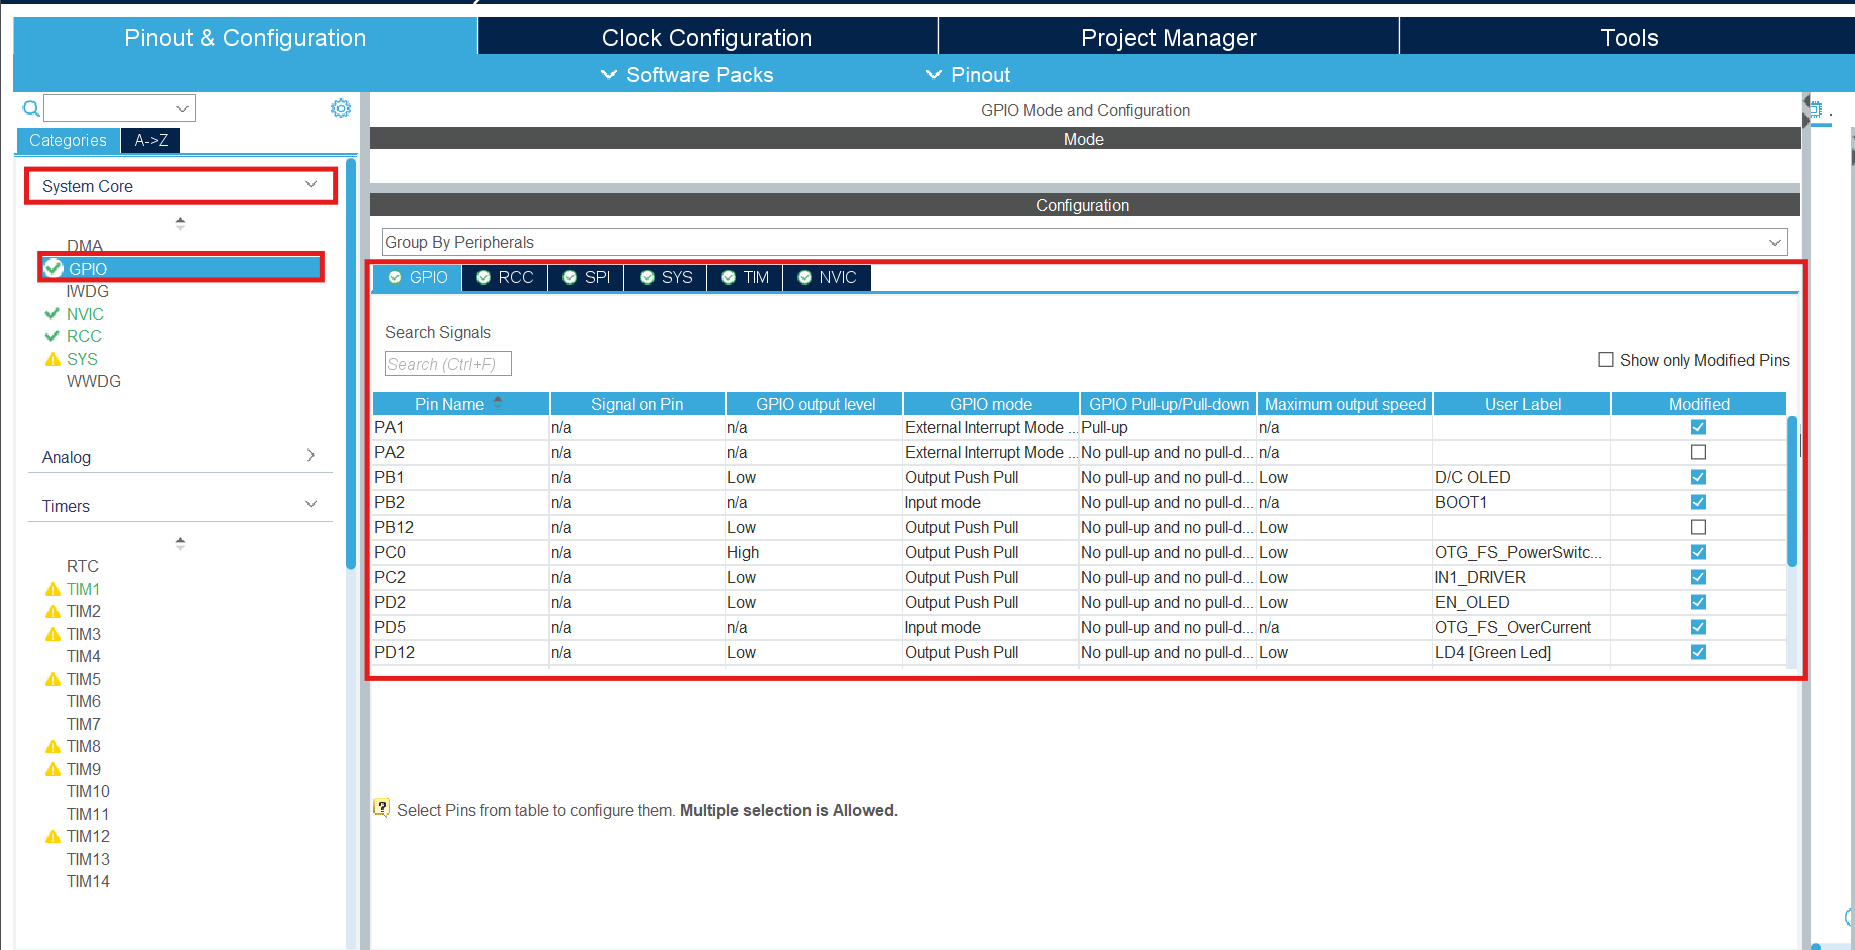
\includegraphics[width=0.75\textwidth]{Perifericos/gpio.png}
    \captionof{figure}{Configuración de GPIOs de control para la OLED y el driver de motor.}
\end{center}

\subsubsection{Configuración de Interrupciones Externas (EXTI)}

Los pulsadores de control del PWM se configuran en modo interrupción:

\begin{itemize}
    \item \textbf{PA1}: External Interrupt, Rising Edge.
    \item \textbf{PA2}: External Interrupt, Rising Edge.
\end{itemize}

Esto permitirá modificar el duty cycle al presionar los botones.  

\begin{center}
    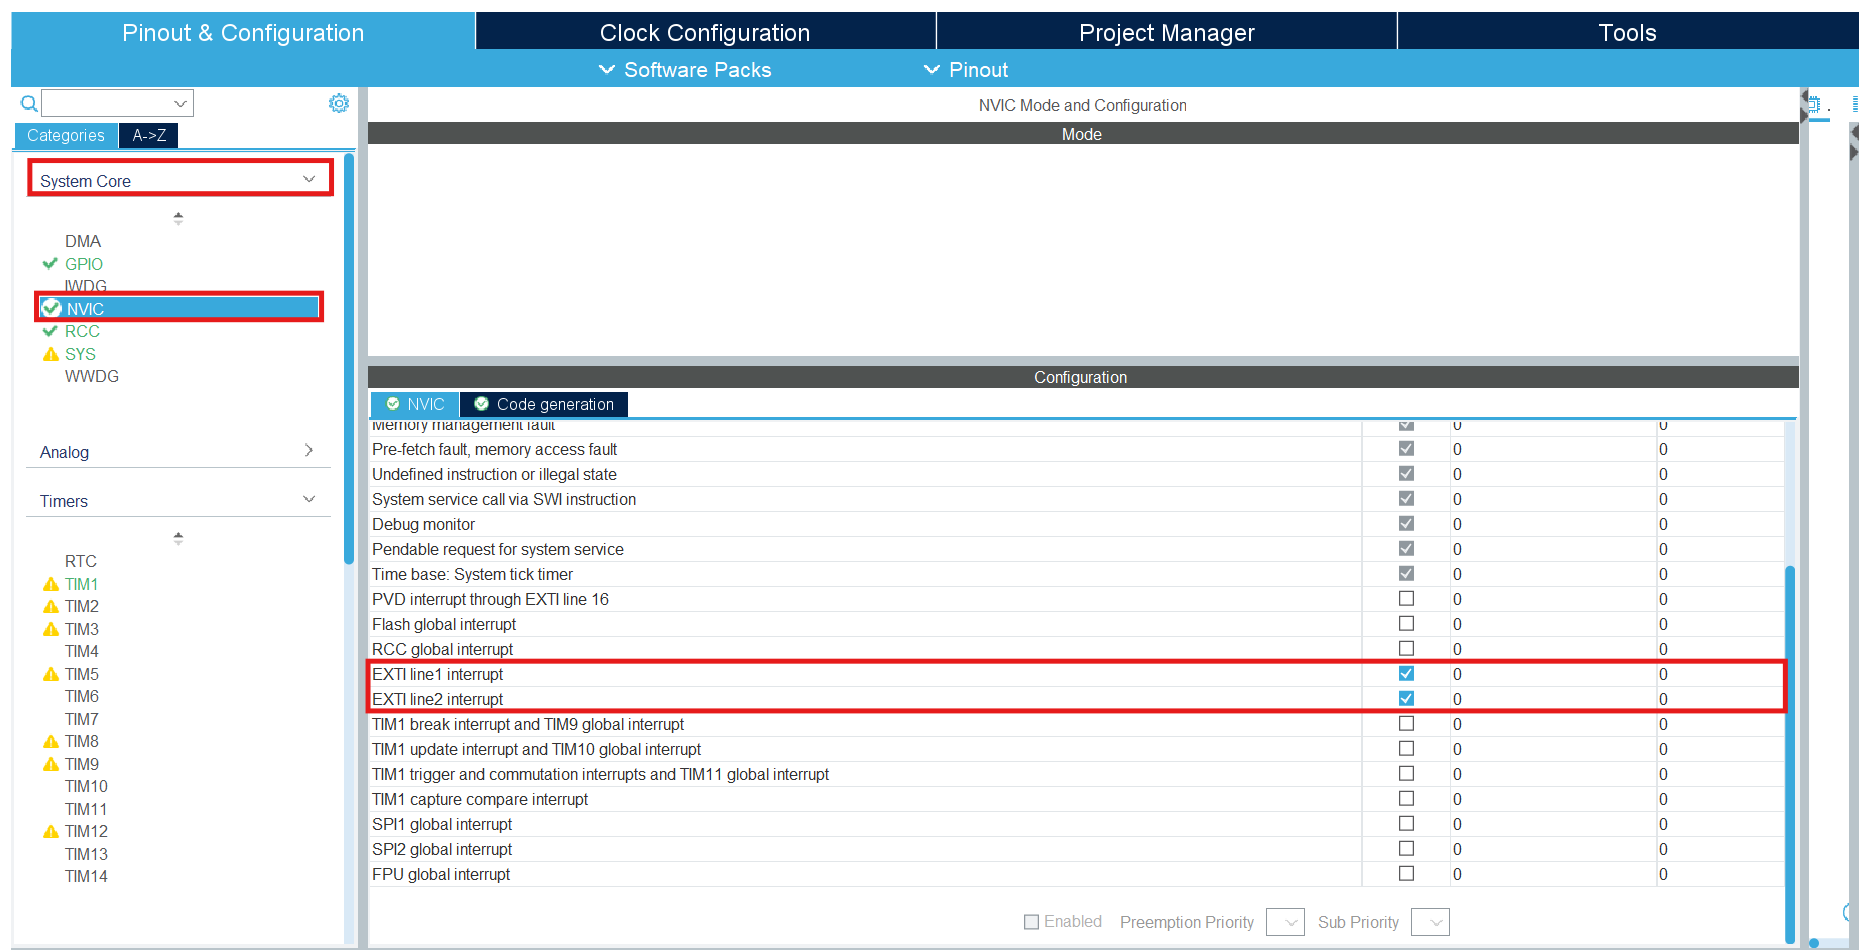
\includegraphics[width=0.75\textwidth]{Perifericos/interrupcion.png}
    \captionof{figure}{Configuración de interrupciones externas para los pulsadores.}
\end{center}

\subsubsection{Configuración del Clock Configuration}

Finalmente, es necesario verificar la pestaña \textbf{Clock Configuration} en CubeMX, la cual permite ajustar la velocidad del sistema y de los periféricos.  
Para esta práctica se recomienda mantener el microcontrolador trabajando a \textbf{84 MHz}, frecuencia suficiente para el manejo simultáneo de SPI, PWM y demás periféricos.

Los pasos son los siguientes:
\begin{enumerate}
    \item Ingresar a la pestaña \textbf{Clock Configuration}.
    \item Seleccionar como fuente principal el \textbf{HSE (High Speed External oscillator)} de 8 MHz presente en la tarjeta STM32F407G-DISC1.
    \item Configurar el \textbf{PLL} de la siguiente forma:
    \begin{itemize}
        \item PLL\_M = 8
        \item PLL\_N = 336
        \item PLL\_P = 4
        \item PLL\_Q = 7
    \end{itemize}
    \item Verificar que la frecuencia del \textbf{SYSCLK} sea de 84 MHz.
    \item Confirmar que las frecuencias derivadas (APB1, APB2, AHB) están dentro de los valores recomendados por el fabricante:
    \begin{itemize}
        \item AHB: 84 MHz
        \item APB1: 42 MHz
        \item APB2: 84 MHz
    \end{itemize}
\end{enumerate}

\begin{center}
    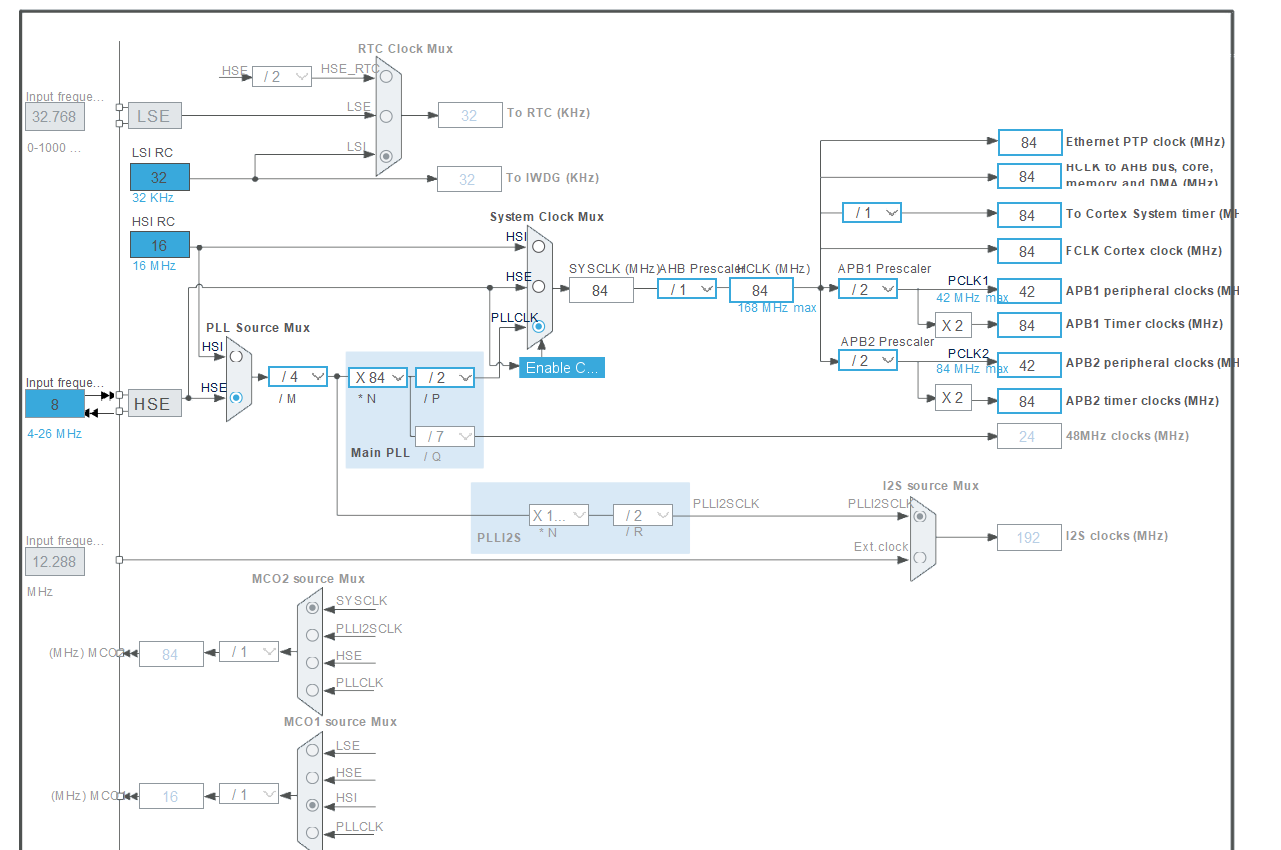
\includegraphics[width=0.85\textwidth]{Perifericos/clock.png}
    \captionof{figure}{Configuración de reloj en CubeMX para trabajar con un SYSCLK de 84 MHz.}
\end{center}

De esta manera, se asegura que los temporizadores (ejemplo: TIM1 para PWM) y las interfaces de comunicación (SPI1 y SPI2) operen con las frecuencias correctas y estables, evitando errores en la transmisión o en el cálculo de periodos.

\subsection{Control de la Pantalla OLED (Librería SSD1351)}

Para manejar la pantalla OLED integrada en la práctica se desarrolló una librería propia, contenida en el archivo \texttt{ssd1351.c}. Esta librería implementa las funciones de inicialización, limpieza de pantalla, escritura de pixeles y renderizado de texto en la pantalla mediante la interfaz \textbf{SPI1}.

A continuación se muestra el código completo del archivo, con un formato que permite visualizarlo de manera similar a como aparece en el entorno de CubeIDE:

\lstset{
    language=C,
    backgroundcolor=\color{black!5},
    basicstyle=\ttfamily\footnotesize,
    keywordstyle=\color{blue}\bfseries,
    stringstyle=\color{red!70!black},
    commentstyle=\color{green!40!black}\itshape,
    numbers=left,
    numberstyle=\tiny,
    stepnumber=1,
    numbersep=5pt,
    tabsize=4,
    showspaces=false,
    showstringspaces=false,
    breaklines=true,
    frame=single,
    captionpos=b
}

\begin{lstlisting}[caption={Implementación de la librería SSD1351 en el archivo \texttt{ssd1351.c}}, label={lst:ssd1351}]
#include <ssd1351.h>
#include "main.h"

extern SPI_HandleTypeDef hspi1;
void SSD1351_DrawPixel(uint8_t x, uint8_t y, uint16_t color);

#define DC_GPIO_Port GPIOB
#define DC_Pin GPIO_PIN_1
#define CS_GPIO_Port GPIOE
#define CS_Pin GPIO_PIN_5
#define RST_GPIO_Port GPIOE
#define RST_Pin GPIO_PIN_4

/* --- Funciones internas para enviar comandos y datos --- */
static void SSD1351_SendCommand(uint8_t cmd) {
    HAL_GPIO_WritePin(DC_GPIO_Port, DC_Pin, GPIO_PIN_RESET);
    HAL_GPIO_WritePin(CS_GPIO_Port, CS_Pin, GPIO_PIN_RESET);
    HAL_SPI_Transmit(&hspi1, &cmd, 1, HAL_MAX_DELAY);
    HAL_GPIO_WritePin(CS_GPIO_Port, CS_Pin, GPIO_PIN_SET);
}

static void SSD1351_SendData(uint8_t *data, uint16_t size) {
    HAL_GPIO_WritePin(DC_GPIO_Port, DC_Pin, GPIO_PIN_SET);
    HAL_GPIO_WritePin(CS_GPIO_Port, CS_Pin, GPIO_PIN_RESET);
    HAL_SPI_Transmit(&hspi1, data, size, HAL_MAX_DELAY);
    HAL_GPIO_WritePin(CS_GPIO_Port, CS_Pin, GPIO_PIN_SET);
}

/* --- Inicializacion del display --- */
void SSD1351_Init(void) {
    HAL_GPIO_WritePin(RST_GPIO_Port, RST_Pin, GPIO_PIN_RESET);
    HAL_Delay(20);
    HAL_GPIO_WritePin(RST_GPIO_Port, RST_Pin, GPIO_PIN_SET);
    HAL_Delay(20);

    SSD1351_SendCommand(0xAE); // Display off
    /* ... Configuracion completa del display ... */
    SSD1351_SendCommand(0xAF); // Display on
}

/* --- Limpiar la pantalla --- */
void SSD1351_Clear(void) {
    SSD1351_SendCommand(0x15);
    SSD1351_SendData((uint8_t[]){0x00, 0x7F}, 2);
    SSD1351_SendCommand(0x75);
    SSD1351_SendData((uint8_t[]){0x00, 0x7F}, 2);
    SSD1351_SendCommand(0x5C);
    uint8_t black[] = {0x00, 0x00};
    for (uint16_t i = 0; i < 128 * 128; i++) {
        SSD1351_SendData(black, 2);
    }
}

/* --- Dibujar un pixel individual --- */
void SSD1351_DrawPixel(uint8_t x, uint8_t y, uint16_t color) {
    if (x >= SSD1351_WIDTH || y >= SSD1351_HEIGHT) return;
    SSD1351_SendCommand(0x15); 
    SSD1351_SendData((uint8_t[]){x, x}, 2);
    SSD1351_SendCommand(0x75);
    SSD1351_SendData((uint8_t[]){y, y}, 2);
    SSD1351_SendCommand(0x5C);
    uint8_t data[2] = {color >> 8, color & 0xFF};
    SSD1351_SendData(data, 2);
}

/* --- Fuente de caracteres 5x8 --- */
const uint8_t font5x8[][5] = {
   /* ... definicion completa de caracteres ... */
};

/* --- Funcion para dibujar texto en pantalla --- */
void SSD1351_DrawText(uint8_t x, uint8_t y, const char *text,
                      uint16_t color, uint16_t bg, uint8_t scale) {
    while (*text) {
        char c = *text++;
        if (c < 32 || c > 127) c = '?';
        const uint8_t *bitmap = font5x8[c - 32];
        /* ... renderizado pixel por pixel ... */
    }
}
\end{lstlisting}

\subsubsection{Explicación del código}

El archivo \texttt{ssd1351.c} se organiza en varias secciones bien diferenciadas:

\begin{itemize}
    \item \textbf{Definición de pines y dependencias}: Se definen los pines de control (\texttt{DC}, \texttt{CS}, \texttt{RST}) que permiten la comunicación con el OLED mediante SPI1.
    \item \textbf{Funciones internas de envío}: \texttt{SSD1351\_SendCommand()} y \texttt{SSD1351\_SendData()} encapsulan la transmisión por SPI, diferenciando entre comandos y datos.
    \item \textbf{Inicialización}: La función \texttt{SSD1351\_Init()} configura el controlador del display paso a paso según su hoja de datos, asegurando que arranque en modo correcto.
    \item \textbf{Funciones gráficas}: 
    \begin{itemize}
        \item \texttt{SSD1351\_Clear()} limpia la pantalla con un color de fondo.
        \item \texttt{SSD1351\_DrawPixel()} permite dibujar un pixel individual en formato \texttt{RGB565}.
    \end{itemize}
    \item \textbf{Fuente de caracteres}: Se incluye una tabla de caracteres 5x8 para poder renderizar texto básico.
    \item \textbf{Dibujo de texto}: \texttt{SSD1351\_DrawText()} recorre la cadena recibida, consultando la fuente y escribiéndola pixel por pixel en pantalla, soportando además escalado.
\end{itemize}

\subsubsection{Archivo de cabecera \texttt{ssd1351.h}}

El archivo de cabecera define las constantes, prototipos de funciones y librerías necesarias para controlar la pantalla OLED SSD1351.  
Este archivo debe guardarse en la carpeta \texttt{Core/Inc} y será incluido posteriormente en el \texttt{main.c}.  

A continuación, se muestra el contenido del archivo:

\newpage

\begin{lstlisting}[language=C, caption={Código del archivo \texttt{ssd1351.h}}, label={cod:ssd1351_h}]
#ifndef __SSD1351_H__
#define __SSD1351_H__

#include "stm32f4xx_hal.h"
#include <stdint.h>

// Resolucion de la pantalla OLED SSD1351
#define SSD1351_WIDTH  128
#define SSD1351_HEIGHT 128

// Prototipos de funciones para el control de la pantalla
void SSD1351_Init(void);
void SSD1351_Clear(void);
void SSD1351_DrawText(uint8_t x, uint8_t y, const char *text,
                      uint16_t color, uint16_t bg, uint8_t scale);

#endif
\end{lstlisting}

\noindent
\textbf{Explicación de los elementos principales:}
\begin{itemize}
    \item \verb|#ifndef ... #define ... #endif|: Esta construcción se denomina \emph{include guard}, y evita que el archivo sea incluido más de una vez en el proyecto, lo cual podría generar errores de compilación.
    \item \verb|#include "stm32f4xx_hal.h"|: Permite el uso de las funciones de la librería HAL específicas del microcontrolador STM32F4.
    \item \verb|#include <stdint.h>|: Incluye definiciones de tipos de datos estándar como \verb|uint8_t| o \verb|uint16_t|, muy usados en programación embebida.
    \item \verb|#define SSD1351_WIDTH 128| y \verb|#define SSD1351_HEIGHT 128|: Constantes que definen la resolución de la pantalla OLED (128x128 píxeles).
    \item \verb|SSD1351_Init()|: Función para inicializar la pantalla OLED (se implementa en \texttt{ssd1351.c}).
    \item \verb|SSD1351_Clear()|: Borra el contenido actual de la pantalla y la rellena con un color de fondo.
    \item \verb|SSD1351_DrawText(...)|: Permite escribir texto en la pantalla, especificando posición (\verb|x, y|), color de texto, color de fondo y tamaño de escala.
\end{itemize}

Este archivo actúa como la \emph{interfaz pública} del controlador, ya que otros archivos del proyecto (como el \texttt{main.c}) podrán usar estas funciones simplemente incluyendo la línea:

\begin{verbatim}
#include "ssd1351.h"
\end{verbatim}


\subsubsection{Creación de archivos adicionales para controladores externos}

En esta práctica no solo se utilizarán los archivos que CubeMX genera de forma automática, sino que también será necesario incluir controladores adicionales, como el de la pantalla OLED SSD1351.  
Estos controladores deben organizarse de forma adecuada dentro del proyecto para que puedan ser incluidos en el \texttt{main.c} y utilizados sin problemas.

Los pasos para crear un nuevo archivo en STM32CubeIDE son los siguientes:

\begin{enumerate}
    \item En el explorador de proyectos (panel izquierdo), ubicar la carpeta llamada \texttt{Core/Src} para los archivos \texttt{.c}, y la carpeta \texttt{Core/Inc} para los archivos \texttt{.h}.
    \item Hacer clic derecho sobre la carpeta correspondiente y seleccionar:
    \begin{itemize}
        \item \texttt{New} $\rightarrow$ \texttt{Source File} para un archivo con extensión \texttt{.c}.
        \item \texttt{New} $\rightarrow$ \texttt{Header File} para un archivo con extensión \texttt{.h}.
    \end{itemize}
    \item Asignar el nombre del archivo, por ejemplo:
    \begin{itemize}
        \item \texttt{ssd1351.c} dentro de la carpeta \texttt{Core/Src}.
        \item \texttt{ssd1351.h} dentro de la carpeta \texttt{Core/Inc}.
    \end{itemize}
    \item En el archivo de cabecera \texttt{ssd1351.h} se definen las funciones, constantes y prototipos necesarios para controlar la pantalla OLED.
    \item En el archivo \texttt{ssd1351.c} se implementa la lógica de dichas funciones (inicialización, limpieza de pantalla, escritura de texto, etc.).
    \item Finalmente, para poder utilizar este controlador en el \texttt{main.c}, se debe incluir la cabecera con:
    \begin{verbatim}
#include "ssd1351.h"
    \end{verbatim}
\end{enumerate}

\begin{center}
    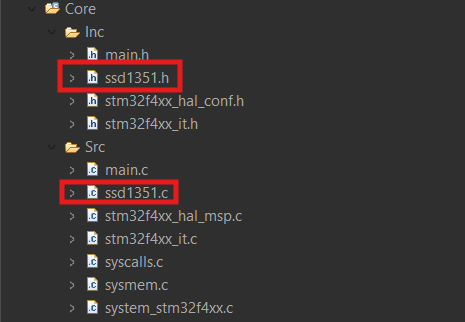
\includegraphics[width=0.85\textwidth]{Librerias/archivos.png}
    \captionof{figure}{Ubicación de archivos adicionales en STM32CubeIDE.}
\end{center}


\subsection{Estructura del archivo \texttt{main.c}}

El archivo principal del proyecto generado por CubeMX (\texttt{main.c}) constituye el núcleo del programa, ya que en él se inicializan los periféricos configurados, se definen las variables globales, se implementan funciones auxiliares y se establece la lógica principal dentro del bucle infinito \texttt{while(1)}.  
A continuación, se desglosan las diferentes partes del código.

\subsubsection{Librerías utilizadas}
En la parte inicial se incluyen tanto las librerías básicas de CubeMX como las adicionales requeridas por la práctica.  

\begin{lstlisting}[language=C, caption={Inclusión de librerías en \texttt{main.c}}]
#include "main.h"
#include <stdio.h>
#include <string.h>
#include "ssd1351.h"
\end{lstlisting}

\begin{itemize}
    \item \verb|main.h|: Cabecera generada automáticamente por CubeMX con las definiciones de pines y periféricos.
    \item \verb|stdio.h| y \verb|string.h|: Librerías estándar de C para funciones de manejo de cadenas y formato.
    \item \verb|ssd1351.h|: Archivo de cabecera creado por el usuario para controlar la pantalla OLED.
\end{itemize}

\subsubsection{Definición de variables y constantes}
En esta sección se declaran los manejadores de periféricos, variables globales y constantes necesarias para el control del sistema.

\begin{lstlisting}[language=C, caption={Variables y constantes en \texttt{main.c}}]
SPI_HandleTypeDef hspi1;
SPI_HandleTypeDef hspi2;
TIM_HandleTypeDef htim1;

#define BLACK   0x0000
#define WHITE   0xFFFF
#define RED     0xF800
#define GREEN   0x07E0
#define BLUE    0x001F
#define YELLOW  0xFFE0

uint32_t last_press_time = 0;  
volatile uint8_t step_count = 0;
const uint8_t duty_steps[6] = {0, 20, 40, 60, 80, 90};
\end{lstlisting}

\begin{itemize}
    \item \verb|hspi1, hspi2|: Manejadores para las interfaces SPI, usados en la OLED y en el sensor de corriente.
    \item \verb|htim1|: Manejador para el temporizador encargado de generar la señal PWM.
    \item Constantes de colores: Representan los valores RGB565 usados para la pantalla OLED.
    \item \verb|last_press_time|: Variable de control para implementar antirrebote en los botones.
    \item \verb|step_count|: Índice de paso para determinar el ciclo de trabajo (\% de PWM).
    \item \verb|duty_steps|: Arreglo con los valores discretos de PWM permitidos en la práctica.
\end{itemize}

\subsection{Funciones implementadas}
En la práctica se definen varias funciones auxiliares para el control del PWM y la lectura de corriente desde el sensor Hall.

\subsubsection*{Control de PWM}
\begin{lstlisting}[language=C]
void Set_PWM_Duty(uint8_t percent) {
    if (percent > 100) return;
    uint32_t pulse = (percent * (__HAL_TIM_GET_AUTORELOAD(&htim1) + 1)) / 100;
    __HAL_TIM_SET_COMPARE(&htim1, TIM_CHANNEL_3, pulse);
}
\end{lstlisting}

Esta función recibe como argumento un porcentaje y ajusta el registro de comparación del temporizador para variar el ciclo de trabajo del PWM.

\subsubsection{Interrupciones por pulsadores}
\begin{lstlisting}[language=C]
void HAL_GPIO_EXTI_Callback(uint16_t GPIO_Pin) {
    if (HAL_GetTick() - last_press_time < 50) return;

    if (GPIO_Pin == GPIO_PIN_1 && step_count < 5) {
        step_count++;
    } else if (GPIO_Pin == GPIO_PIN_2 && step_count > 0) {
        step_count--;
    }
    Set_PWM_Duty(duty_steps[step_count]);
    last_press_time = HAL_GetTick();
}
\end{lstlisting}

Aquí se controla el incremento o decremento del PWM mediante botones conectados a los pines \verb|PA1| y \verb|PA2|, incluyendo un filtro de software para el antirrebote.

\newpage

\subsubsection{Lectura del sensor de corriente}
\begin{lstlisting}[language=C]
int16_t Read_Current_Signed(void) {
    uint8_t tx_dummy[2] = {0x00, 0x00};
    uint8_t rx_data[2] = {0};

    HAL_GPIO_WritePin(GPIOB, GPIO_PIN_12, GPIO_PIN_RESET); // CS LOW
    HAL_SPI_TransmitReceive(&hspi2, tx_dummy, rx_data, 2, HAL_MAX_DELAY);
    HAL_GPIO_WritePin(GPIOB, GPIO_PIN_12, GPIO_PIN_SET);   // CS HIGH

    uint16_t raw = ((uint16_t)rx_data[0] << 8) | rx_data[1];
    int16_t current_raw = raw & 0x1FFF;
    if (current_raw & 0x1000) {
        current_raw |= 0xE000; // Extiende signo
    }
    return current_raw;
}
\end{lstlisting}

La función lee dos bytes por SPI desde el sensor Hall de corriente y procesa los datos para devolver un valor con signo.

\subsection{Desglose del archivo \texttt{main.c}}

En esta sección se explicará la estructura del archivo principal del proyecto, mostrando de manera ordenada el uso de librerías, variables globales, funciones auxiliares, la función \texttt{main()} y el bucle infinito \texttt{while}.

\subsubsection{Librerías utilizadas}

Las librerías incluidas en este proyecto permiten acceder a las funciones de la HAL (Hardware Abstraction Layer) de STM32 y a utilidades estándar como \texttt{stdio.h} para depuración.

\begin{lstlisting}[language=C, caption={Librerías incluidas en \texttt{main.c}}, label={cod:libs}]
#include "main.h"
#include <stdio.h>
\end{lstlisting}

\begin{itemize}
    \item \texttt{main.h}: Archivo de cabecera generado por CubeMX que contiene la configuración de pines, macros y prototipos.
    \item \texttt{stdio.h}: Usado para redirigir funciones como \texttt{printf()} hacia la UART.
\end{itemize}


\subsubsection{Definición de variables}

Se definen estructuras de la HAL para manejar periféricos, así como variables para el control del PWM y el sensor de corriente.

\begin{lstlisting}[language=C, caption={Variables globales}, label={cod:variables}]
SPI_HandleTypeDef hspi1;
UART_HandleTypeDef huart2;
TIM_HandleTypeDef htim1;

uint32_t last_press_time = 0;  // Antirrebote
volatile uint8_t step_count = 0;

// Escalones de duty cycle en %
const uint8_t duty_steps[6] = {0, 20, 40, 60, 80, 90};
\end{lstlisting}

\begin{itemize}
    \item \texttt{hspi1}, \texttt{huart2}, \texttt{htim1}: Estructuras de la HAL que almacenan la configuración activa de SPI, UART y Timer.
    \item \texttt{last\_press\_time}: Control de tiempo para evitar rebotes en el botón.
    \item \texttt{step\_count}: Índice del nivel de PWM actual.
    \item \texttt{duty\_steps}: Arreglo con los valores de duty cycle disponibles.
\end{itemize}


\subsubsection{Funciones auxiliares}

El código define varias funciones que facilitan el manejo de periféricos.  

\begin{lstlisting}[language=C, caption={Funciones auxiliares}, label={cod:funciones}]
void Set_PWM_Duty(uint8_t percent) {
    if (percent > 100) return;
    uint32_t pulse = (percent * (__HAL_TIM_GET_AUTORELOAD(&htim1) + 1)) / 100;
    __HAL_TIM_SET_COMPARE(&htim1, TIM_CHANNEL_1, pulse);
}

void HAL_GPIO_EXTI_Callback(uint16_t GPIO_Pin) {
    if (GPIO_Pin == GPIO_PIN_1) {
        if (HAL_GetTick() - last_press_time > 50) { // Antirrebote
            step_count = (step_count + 1) % 6;
            Set_PWM_Duty(duty_steps[step_count]);
            last_press_time = HAL_GetTick();
        }
    }
}

uint16_t Read_Current_Raw(void) {
    uint8_t tx_dummy[2] = {0x00, 0x00};
    uint8_t rx_data[2] = {0};

    HAL_GPIO_WritePin(GPIOA, GPIO_PIN_4, GPIO_PIN_RESET); // CS LOW
    HAL_SPI_TransmitReceive(&hspi1, tx_dummy, rx_data, 2, HAL_MAX_DELAY);
    HAL_GPIO_WritePin(GPIOA, GPIO_PIN_4, GPIO_PIN_SET);   // CS HIGH

    uint16_t raw = ((uint16_t)rx_data[0] << 8) | rx_data[1];
    return raw & 0x0FFF;  // 12 bits validos
}

// Redirigir printf al puerto serie
int __io_putchar(int ch) {
    HAL_UART_Transmit(&huart2, (uint8_t *)&ch, 1, HAL_MAX_DELAY);
    return ch;
}
\end{lstlisting}

\begin{itemize}
    \item \texttt{Set\_PWM\_Duty}: Ajusta el ciclo útil del PWM en base a un valor porcentual.
    \item \texttt{HAL\_GPIO\_EXTI\_Callback}: Rutina de interrupción para el pulsador que incrementa el duty cycle.
    \item \texttt{Read\_Current\_Raw}: Lee 12 bits crudos del sensor de corriente a través de SPI.
    \item \texttt{\_\_io\_putchar}: Redirige \texttt{printf()} hacia la UART2.
\end{itemize}


\subsubsection{Función \texttt{main()} y bucle infinito}

El \texttt{main()} realiza la inicialización de periféricos, configura el reloj del sistema y entra en el bucle \texttt{while(1)}, donde ocurre la lógica principal.

\begin{lstlisting}[language=C, caption={Fragmento de la función \texttt{main}}, label={cod:main}]
int main(void)
{
  HAL_Init();               // Inicializacion de la HAL
  SystemClock_Config();     // Configuracion de reloj
  MX_GPIO_Init();
  MX_SPI1_Init();
  MX_USART2_UART_Init();
  MX_TIM1_Init();

  // Iniciar PWM en canal 1
  HAL_TIM_PWM_Start(&htim1, TIM_CHANNEL_1);
  Set_PWM_Duty(0);  // Arranca en 0%

  while (1)
  {
      uint32_t suma_raw = 0;
      for (int i = 0; i < 10; i++) {
          suma_raw += Read_Current_Raw();
          HAL_Delay(10);
      }

      uint16_t raw_promedio = suma_raw / 10;
      float current_mA = (raw_promedio - 2049) * 25.0f;

      // Imprimir resultados
      printf("Corriente Promedio: %.2f mA | Raw: %u | PWM Duty: %u%%\r\n",
             current_mA, raw_promedio, duty_steps[step_count]);

      // Ajuste automatico de PWM
      if (current_mA > 100.0f && step_count < 5) {
          step_count++;
          Set_PWM_Duty(duty_steps[step_count]);
          printf("PWM aumentado a %u%% por corriente alta.\r\n", duty_steps[step_count]);
      }

      HAL_Delay(1000);  // 1 segundo entre mediciones
  }
}
\end{lstlisting}

\begin{itemize}
    \item Se inicializan todos los periféricos generados por CubeMX (\texttt{GPIO}, \texttt{SPI1}, \texttt{UART2}, \texttt{TIM1}).
    \item El PWM inicia en 0\% y se incrementa por medio del pulsador o automáticamente si la corriente medida supera un umbral.
    \item Cada segundo se promedian 10 muestras del sensor y se calcula la corriente.
    \item Los datos son enviados por UART para monitoreo en consola.
\end{itemize}


\section{Análisis del archivo \texttt{main.c}}

En este apartado se presenta el desglose del archivo principal del proyecto, \texttt{main.c}.  
El objetivo es comprender la lógica detrás de la inicialización, la organización de funciones y el bucle principal que gobierna la práctica.

\subsection{Inclusión de librerías}
El archivo comienza incluyendo tanto librerías estándar como específicas del microcontrolador.  

\begin{lstlisting}[language=C]
#include "main.h"
#include <stdio.h>
#include <string.h>
#include "ssd1351.h"
\end{lstlisting}

\begin{itemize}
    \item \texttt{main.h}: Generado automáticamente por CubeMX, contiene definiciones de pines y prototipos básicos.
    \item \texttt{stdio.h} y \texttt{string.h}: Librerías estándar de C para manejo de cadenas y funciones de formato.
    \item \texttt{ssd1351.h}: Controlador externo desarrollado para la pantalla OLED.
\end{itemize}

\subsection{Definiciones de variables y constantes}
En esta sección se encuentran las variables globales, estructuras de configuración de periféricos y constantes de uso general.  

\begin{lstlisting}[language=C]
SPI_HandleTypeDef hspi1;
SPI_HandleTypeDef hspi2;
TIM_HandleTypeDef htim1;

#define BLACK   0x0000
#define WHITE   0xFFFF
#define RED     0xF800
#define GREEN   0x07E0
#define BLUE    0x001F
#define YELLOW  0xFFE0

uint32_t last_press_time = 0;  // Antirrebote
volatile uint8_t step_count = 0;
const uint8_t duty_steps[6] = {0, 20, 40, 60, 80, 90};
\end{lstlisting}

\begin{itemize}
    \item \textbf{Colores}: definidos en formato RGB565, compatibles con la OLED.
    \item \textbf{last\_press\_time}: almacena la última pulsación para implementar antirrebote.
    \item \textbf{step\_count}: índice que controla el nivel de PWM actual.
    \item \textbf{duty\_steps}: tabla de posibles valores de ciclo de trabajo (\%) para el PWM.
\end{itemize}

\subsection{Funciones auxiliares}
Se implementan funciones que encapsulan comportamientos específicos como ajuste de PWM, interrupciones y lectura del sensor de corriente.

\subsubsection*{Ajuste de ciclo de trabajo PWM}
\begin{lstlisting}[language=C]
void Set_PWM_Duty(uint8_t percent) {
    if (percent > 100) return;
    uint32_t pulse = (percent * (__HAL_TIM_GET_AUTORELOAD(&htim1) + 1)) / 100;
    __HAL_TIM_SET_COMPARE(&htim1, TIM_CHANNEL_3, pulse);
}
\end{lstlisting}
Esta función calcula el valor del registro de comparación para fijar el ciclo útil de la señal PWM.

\subsubsection*{Interrupción por pulsadores}
\begin{lstlisting}[language=C]
void HAL_GPIO_EXTI_Callback(uint16_t GPIO_Pin) {
    if (HAL_GetTick() - last_press_time < 50) return;  // Antirrebote

    if (GPIO_Pin == GPIO_PIN_1 && step_count < 5) {
        step_count++;
    } else if (GPIO_Pin == GPIO_PIN_2 && step_count > 0) {
        step_count--;
    }

    Set_PWM_Duty(duty_steps[step_count]);
    last_press_time = HAL_GetTick();
}
\end{lstlisting}
Permite incrementar o decrementar el ciclo útil mediante interrupciones de los pines \texttt{PA1} y \texttt{PA2}.

\subsubsection*{Lectura del sensor de corriente}
Se implementan funciones para comunicarse con el sensor a través del bus SPI2.

\begin{lstlisting}[language=C]
uint16_t Read_Current_Raw(void) { ... }
int16_t Read_Current_Signed(void) { ... }
\end{lstlisting}

Ambas realizan una transacción SPI y reconstruyen el valor de 13 bits que entrega el sensor Hall de corriente.

\subsection{Función principal \texttt{main()}}
La función \texttt{main} organiza la ejecución del programa. Primero inicializa el hardware, luego configura periféricos y finalmente entra en el bucle infinito.

\begin{enumerate}
    \item Inicialización de HAL y reloj del sistema.
    \item Configuración de periféricos: GPIO, SPI1, SPI2, TIM1.
    \item Encendido del PWM en el canal 3 de TIM1.
    \item Activación de pines de control para el driver de motor y la OLED.
    \item Inicialización de la pantalla OLED y limpieza de contenido.
\end{enumerate}

\subsection{Bucle \texttt{while(1)}}
El ciclo infinito contiene la lógica de la práctica:

\newpage

\begin{lstlisting}[language=C]
while (1) {
    uint32_t suma_raw = 0;
    for (int i = 0; i < 10; i++) {
        suma_raw += Read_Current_Raw();
        HAL_Delay(10);
    }

    uint16_t raw_prom = suma_raw / 10;
    float current_mA = (raw_prom - 2048) * 25.0f;

    snprintf(buffer_current, sizeof(buffer_current), "I: %.1fmA", current_mA);
    snprintf(buffer_duty, sizeof(buffer_duty), "D: %u%%", duty_steps[step_count]);

    SSD1351_Clear();
    SSD1351_DrawText(10, 10, buffer_current, BLUE, BLACK, 2);
    SSD1351_DrawText(10, 30, buffer_duty, BLUE, BLACK, 2);

    if (current_mA > 100.0f && step_count < 5) {
        step_count++;
        Set_PWM_Duty(duty_steps[step_count]);
    }

    HAL_Delay(1000);
}
\end{lstlisting}

\noindent
\textbf{Flujo general:}
\begin{enumerate}
    \item Se promedian 10 lecturas consecutivas del sensor para reducir ruido.
    \item Se convierte la lectura cruda en corriente (mA).
    \item Se actualiza la pantalla OLED con el valor de corriente y el ciclo de trabajo.
    \item Se implementa una condición de protección: si la corriente supera 100 mA, se aumenta automáticamente el ciclo útil.
    \item Se repite el proceso cada segundo.
\end{enumerate}


\section{Resultados}

En esta sección se presentan los resultados obtenidos al implementar el sistema de medición de corriente, control de PWM y visualización en pantalla OLED utilizando la tarjeta \textbf{STM32F407G-DISC1} y la Discovery Shield.  

Se configuró el generador PWM con un ciclo de trabajo del \textbf{90\%}, lo que permitió alcanzar una velocidad elevada en el motor y, en consecuencia, un mayor consumo de corriente. Estos valores fueron correctamente medidos por el sensor de corriente Hall y mostrados en la pantalla OLED, confirmando el correcto funcionamiento del sistema integrado.

\begin{figure}[H]
    \centering
    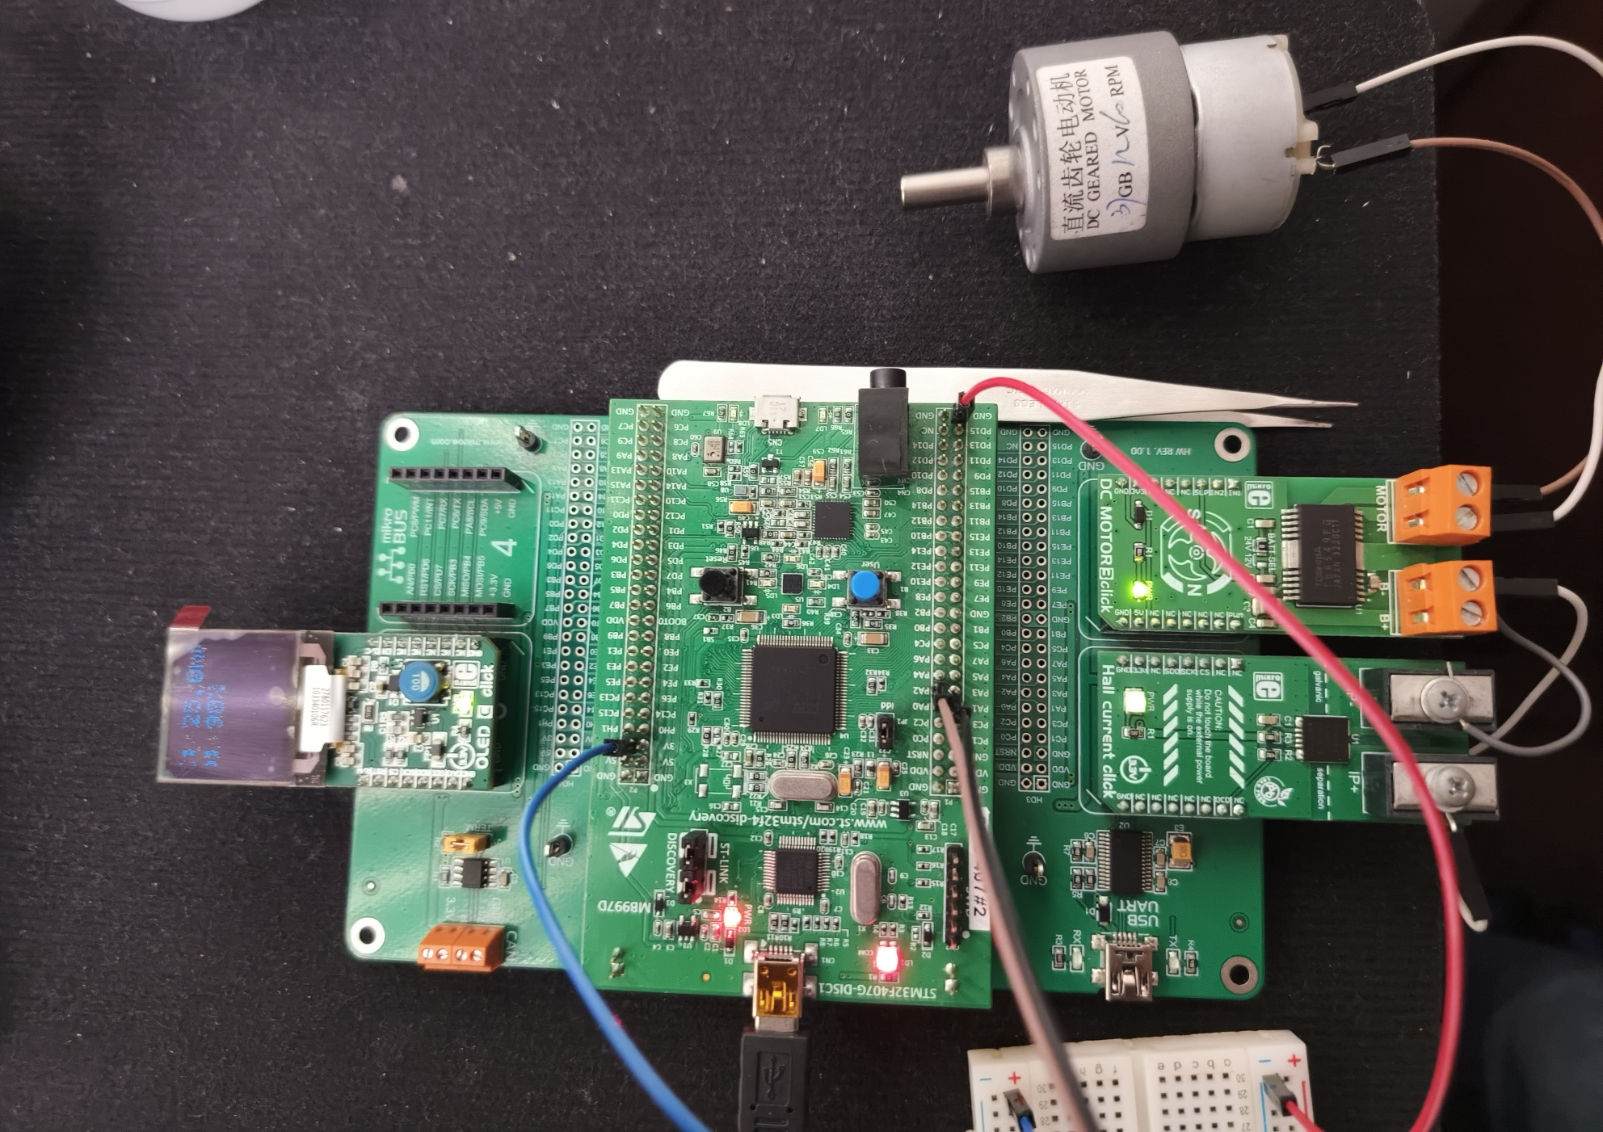
\includegraphics[width=0.65\textwidth]{Resultados/90.png}
    \caption{Visualización en pantalla OLED y comportamiento del motor con un ciclo de trabajo del 90\%.}
    \label{fig:resultados_pwm_90}
\end{figure}

El resultado evidencia que el sistema responde de manera adecuada al incremento en el ciclo de trabajo, mostrando en la pantalla OLED el valor de la corriente consumida y reflejando en el motor un régimen de operación de alta velocidad.




\end{document}
